\chapter{Datenreduktion der Fokusserien}
\label{chapter_2}
Die in diesem Kapitel beschriebenen Schritte wurden in kleinen Programmen mithilfe der Programmiersprache Python implementiert. Eine ausgiebige Dokumentation der Funktionen sowie deren Gebrauch findet sich im Softwarerepositorium gemeinsam mit dem Quelltext.\\
An dieser Stelle sollen die von den Programmen erstellten Plots nur exemplarisch präsentiert werden, um die Übersichtlichkeit nicht zu beeinträchtigen. Im Anhang findet sich eine vollständige Übersicht aller Parameter und ihrer Plots.

\section{Diskrete Dichteverteilungsfunktionen}
In einem ersten Schritt wurden die Daten der Fokusserien aufbereitet um diskrete Verteilungsfunktionen zu erhalten. Für jede Aufnahme stand ein Satz an Teleskop-spezifischen Meta-Parametern (TSI-Parameter) sowie eine Liste aller Sterne und ihre Pixel-Position sowie Abberations-Koeffizieten (PSF-Parameter), wie in Kapitel 1 beschrieben, zur Verfügung.\\
Die PSF-Parameter wurden für jede Aufnahme auf ihren Median reduziert. Um dennoch womögliche Unterschiede in der Position auf dem Detektor-Mosaik feststellen zu können, wird jede Aufnahme in ein $3\times 3$ aufgeteilt und jedem Quadrat im Gitter der Median der jeweiligen Sterne im Quadrat zugeteilt. Das Ergebnis sind Verteilungsfunktionen aller PSF-Parameter für 9 quadratische Bildbereiche auf dem Detektor (Abb. \ref{a4_dist}).\\
Für die Distributionen der TSI-Parameter war keine weitere Reduktion nötig (Abb. \ref{tsi_temp}). Allerdings wurden aufgrund der hohen Anzahl der Parameter statische und quasi-statische Parameter entfernt. Als quasi-statisch wurden solche Parameter interpretiert, deren Werte bei einem Binning von 50 zu $\ge\SI{95}{\percent}$ auf einen Wert fallen.
\vfill\,

\begin{figure}[H]
	\centering
	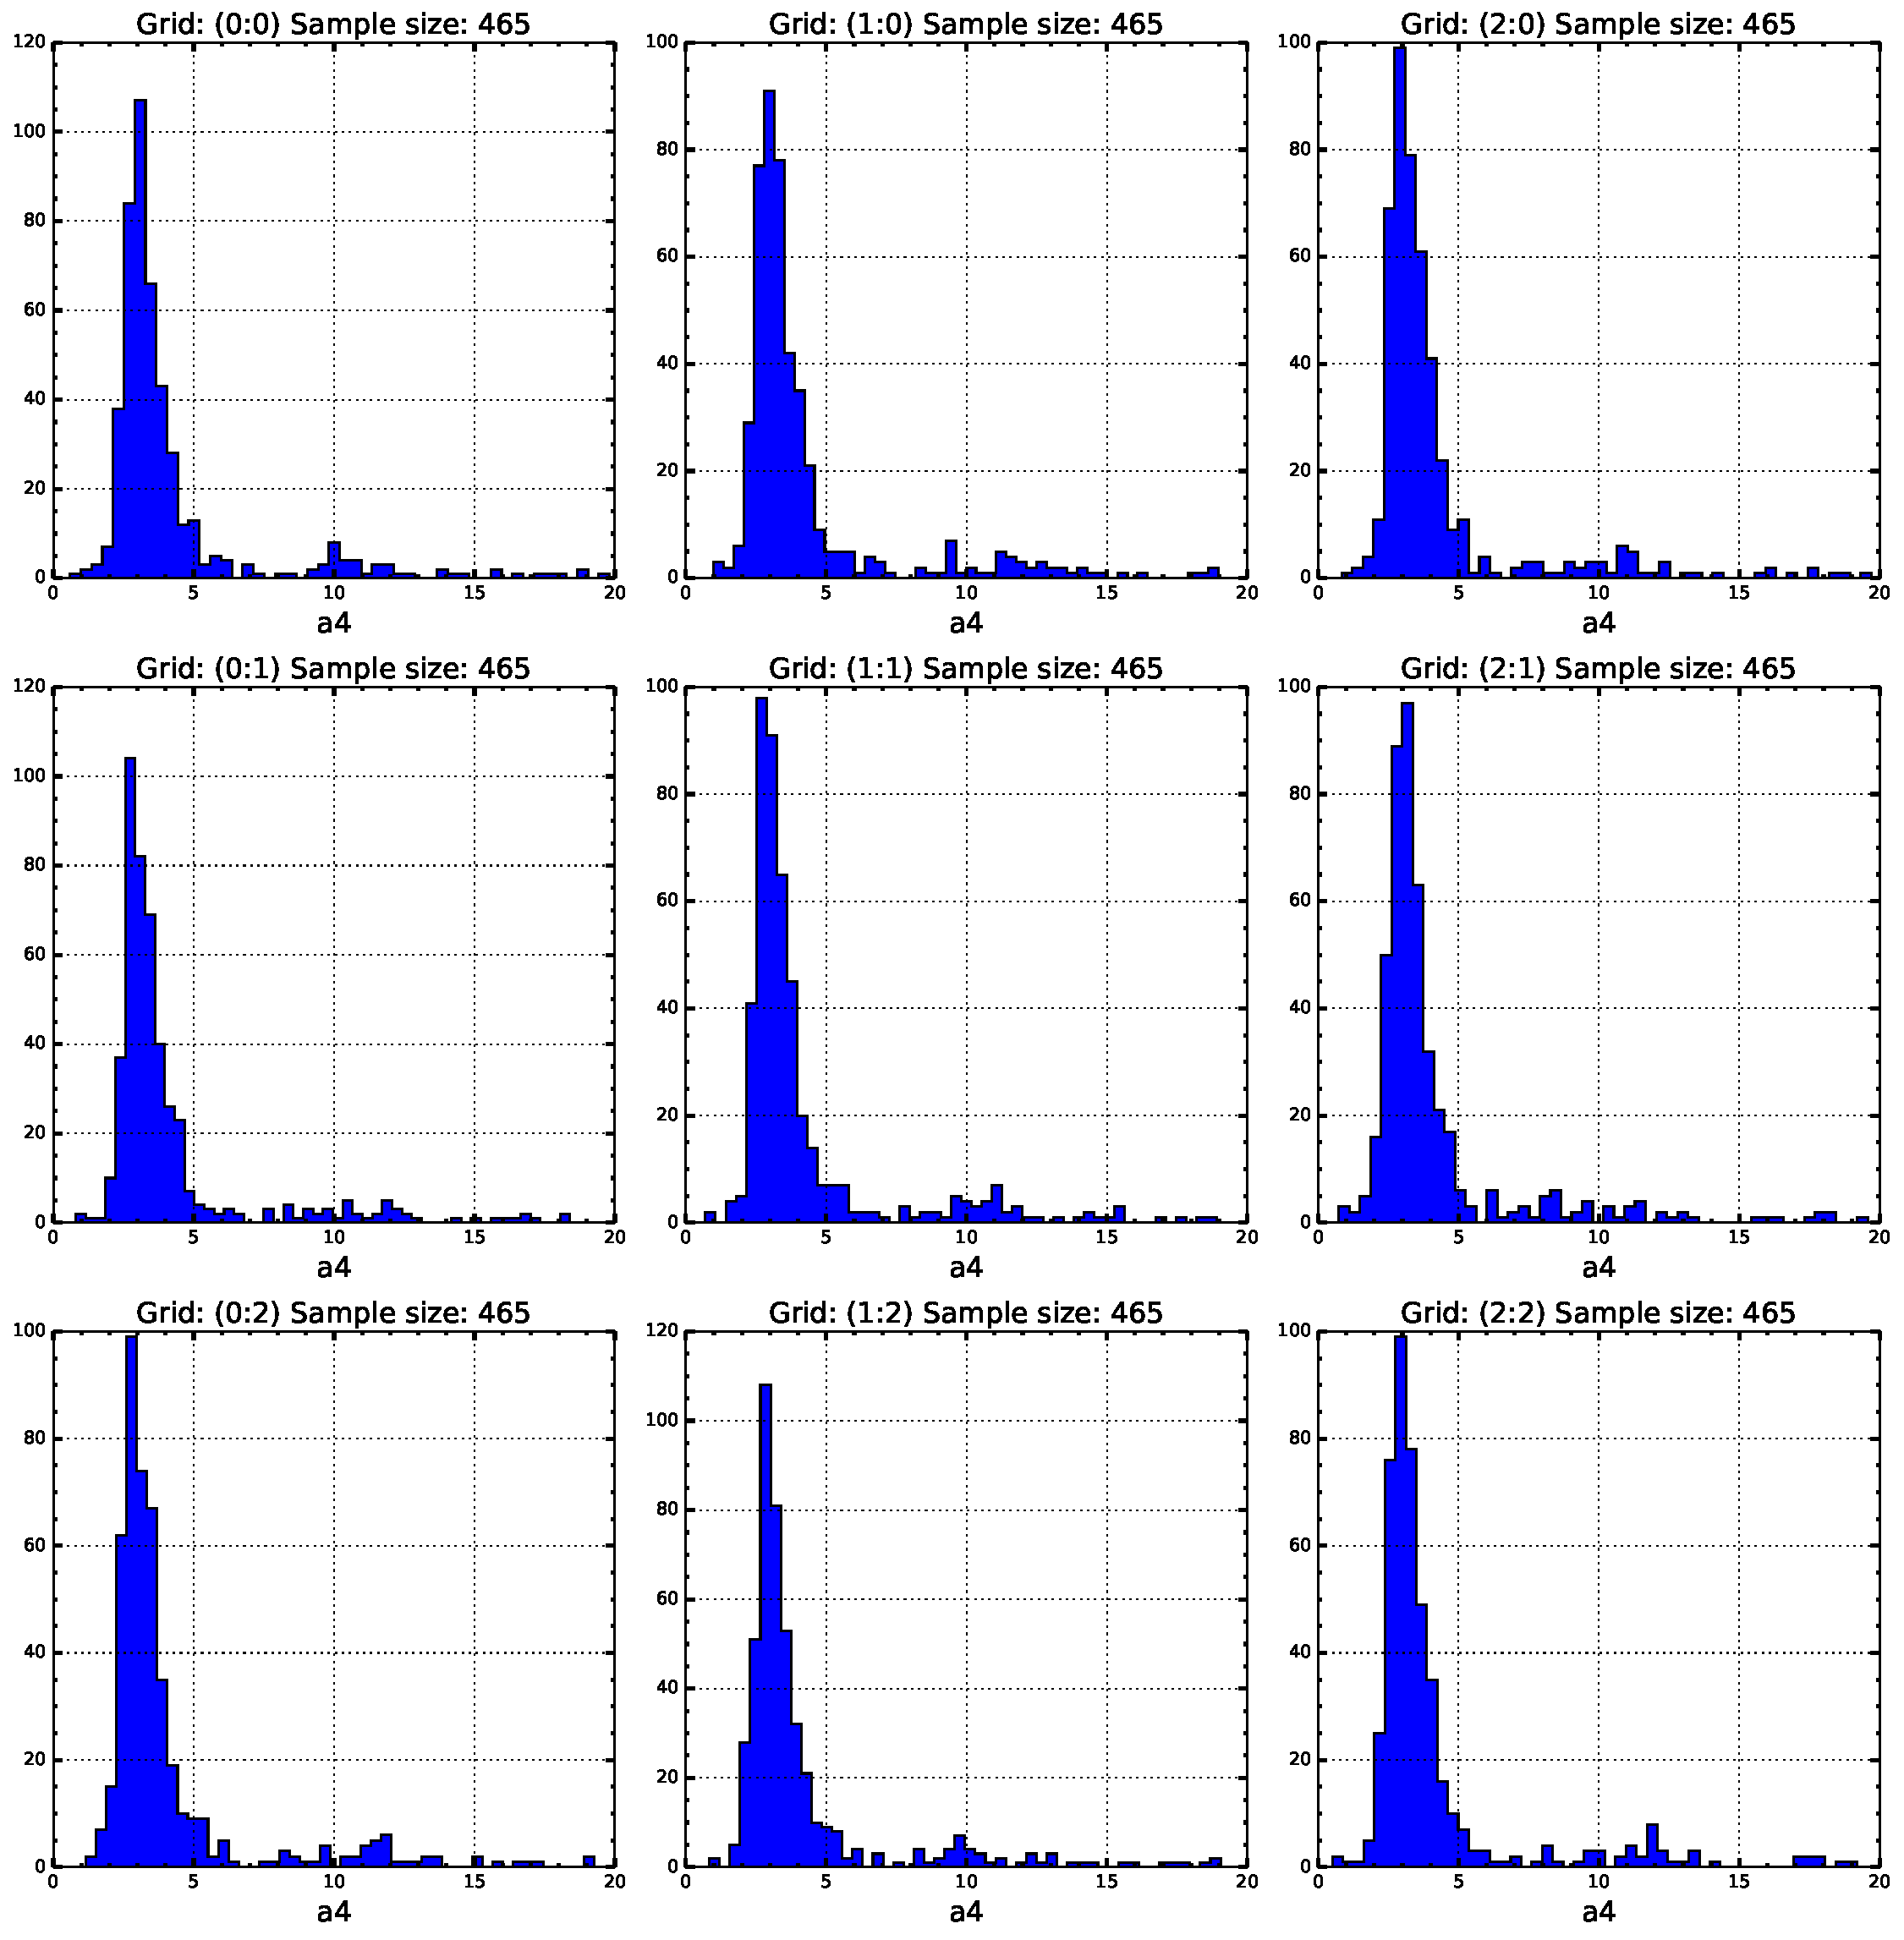
\includegraphics[scale=.40]{psf_dist/a4.pdf}
	\caption[Diskrete Verteilungsfunktionen des PSF-Parameters $A_4$]{Diskrete Verteilungsfunktionen des PSF-Parameters $A_4$. Die Lage des Plots in der Grafik entspricht der Gitter-Position des Quadrats auf dem Detektor. Zugrunde liegen die Daten der ausgewählten Fokus-Aufnahmen aus 465 Fokusserien. Für den Plot wurde der Definitionsbereich in 50 gleichgroße Teilstücke geteilt und die Werte in den Teilstücken gezählt (sog. \emph{Binning}).}
    \label{a4_dist}
\end{figure}

\begin{figure}[H]
	\centering
	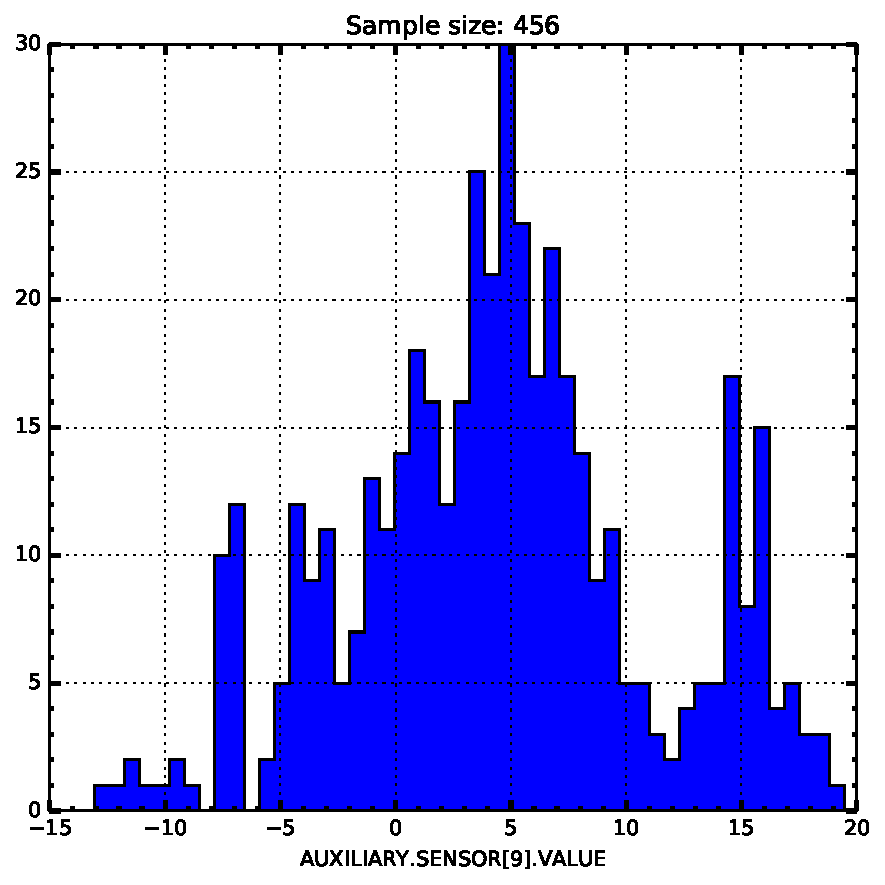
\includegraphics[scale=.75]{tsi_dist/AUXILIARY_SENSOR_9__VALUE.pdf}
	\caption[Diskrete Verteilungsfunktion eines Temperatursensors]{Diskrete Verteilungsfunktion eines Temperatursensors. Zugrunde liegen die Daten der ausgewählten Fokus-Aufnahmen aus 456 Fokusserien. Binning: 50.}
    \label{tsi_temp}
\end{figure}

\section{Transinformation der Aberrations-Koeffizieten sowie der Teleskop Meta-Daten}

Um zu überprüfen ob es weitere Abhängigkeiten im Teleskop-System gibt, die sich auf den Fokus auswirken, wurden alle Verteilungsfunktionen (sowohl PSF- als auch TSI-Parameter) miteinander verglichen und ein normierter Transinformations-Index berechnet.\\
Diese Information liegt zunächst tabelliert vor. Damit sie effektiv betrachtet und analysiert werden kann, wurde sie in eine Korrelationsmatrix eingetragen und in einem Heatmap-Diagramm geplottet (Abb. \ref{psf_heatmap}).

\begin{figure}[H]
	\centering
	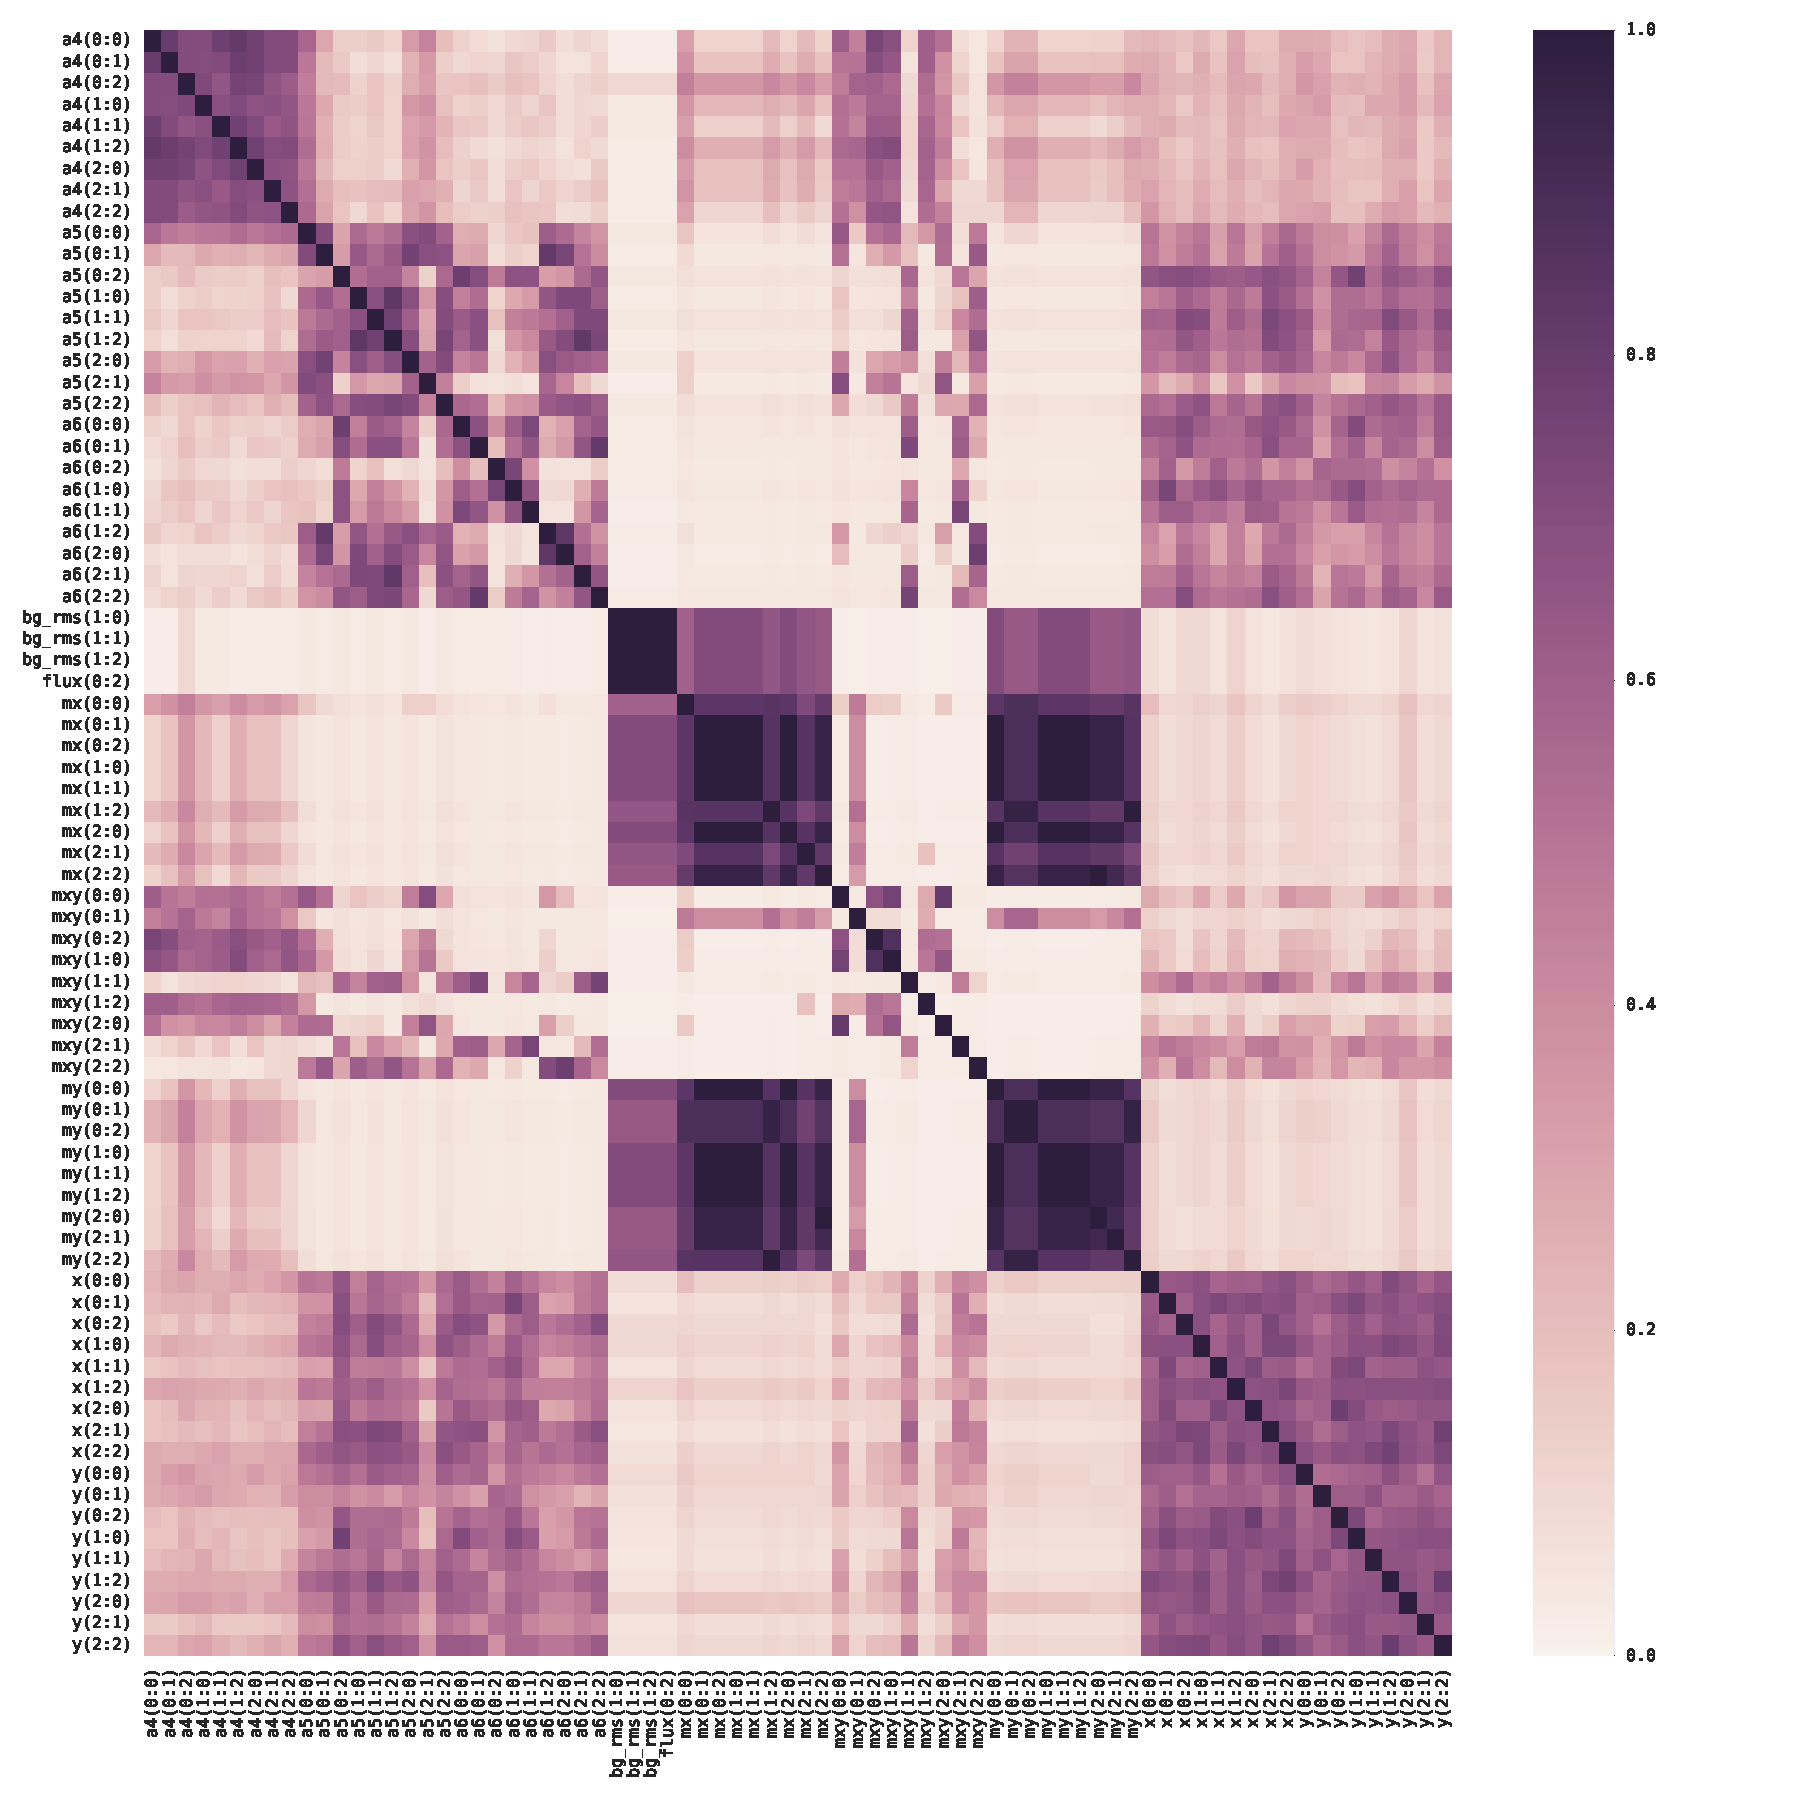
\includegraphics[scale=.56]{heatmaps/psf.pdf}
	\caption[Transinformations-Heatmap der PSF-Parameter]{Transinformations-Heatmap der PSF-Parameter. Jeder Pixel auf der Karte entspricht einem normierten Transinformations-Index. Da beide Achsen die selben Parameter enthalten nimmt jeder Wert auf der Diagonalen den Wert $\num{1}$ an.}
    \label{psf_heatmap}
\end{figure}

\section{Einfluss der Windgeschwindigkeit und Windrichtung}
Vor dem Bau des Fraunhofer Teleskops konnten bereits gute Beobachtungsbedingungen, insbesondere Seeing, am Wendelstein Observatorium nachgewiesen werden\cite{wendelstein_seeing}. Dennoch wurde ein Werkzeug entwickelt, um den Zusammenhang zwischen schlechter Bildqualität und Windgeschwindigkeit sowie Windrichtung auswerten zu können. Hierzu wurden aus den meteologischen Logdateien für jede Fokusaufnahme die relevanten Windwerte extrahiert und mit den PSF-Mittelwerten der Aufnahme verknüpft. Somit lassen sich die PSF-Parameter in Abhängigkeit von Windgeschwindigkeit, Windrichtung und Temperatur darstellen und auf mögliche Muster überprüfen (Abb. \ref{wind_a4}).

\begin{figure}[h]
	\centering
	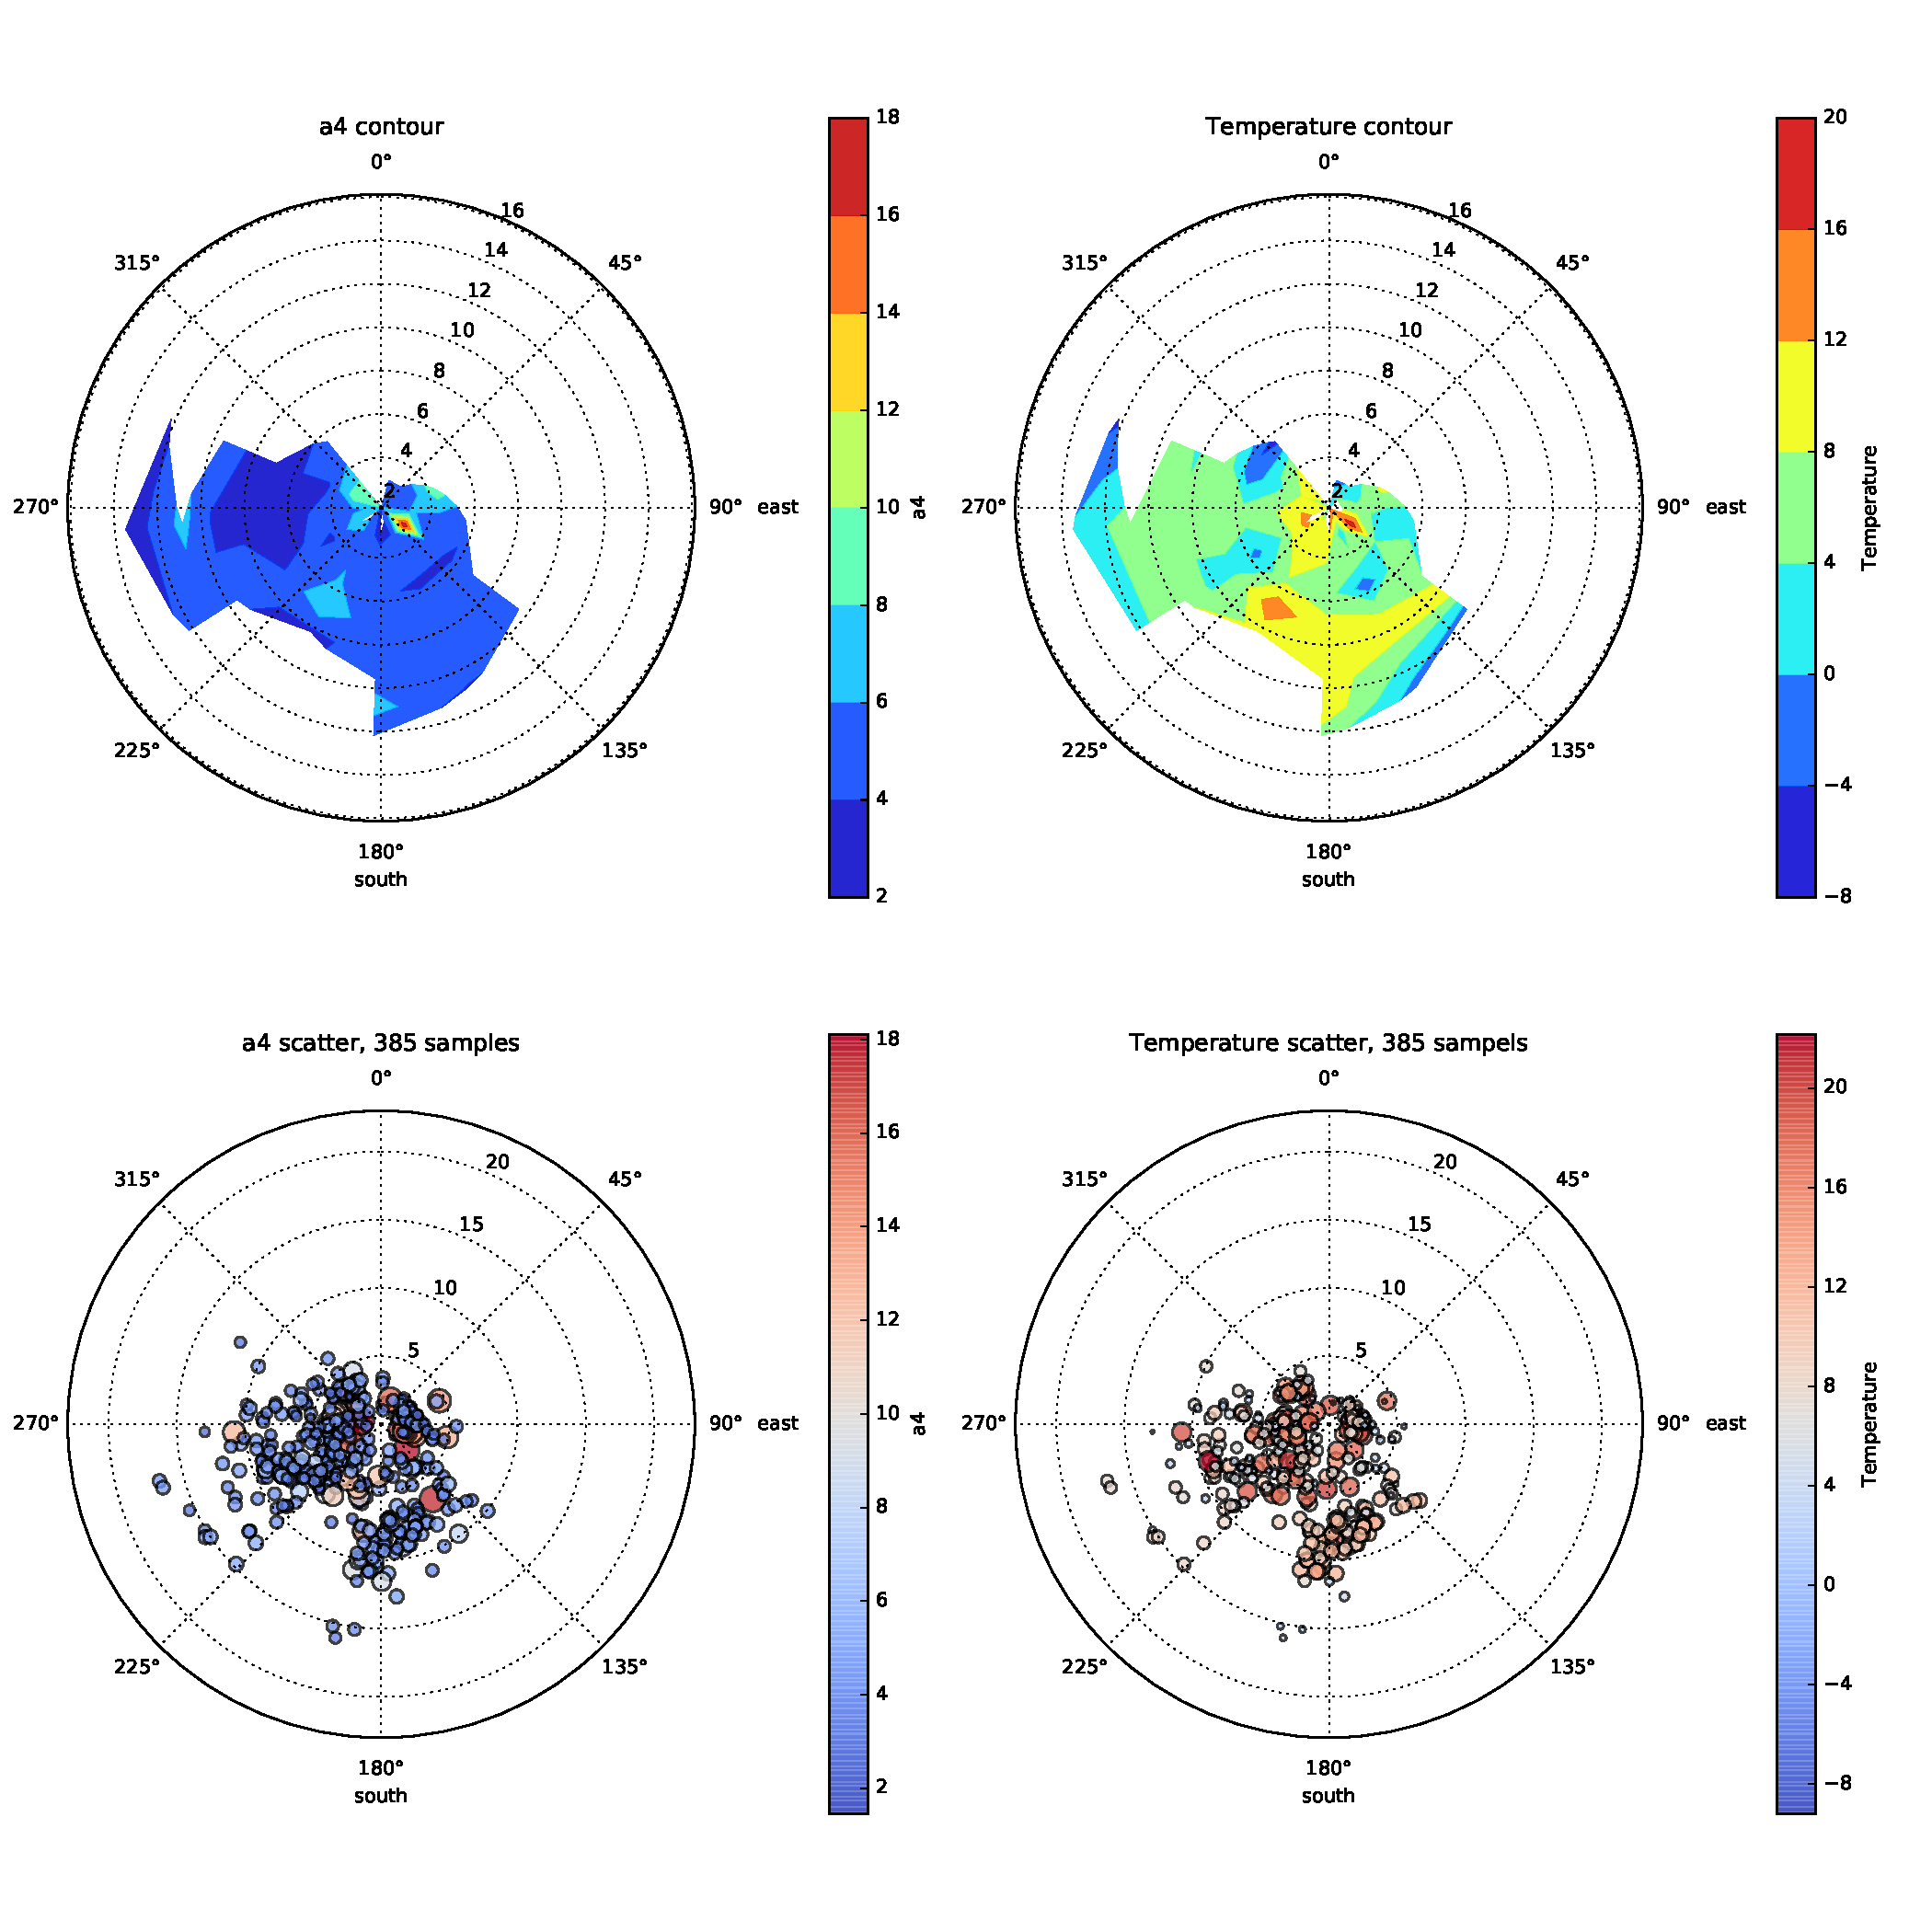
\includegraphics[scale=.48]{wind/wind_a4.pdf}
	\caption[Einfluss von Windgeschwindigkeit und Windrichtung auf $A_4$]{Einfluss von Windgeschwindigkeit und Windrichtung auf $A_4$. Die Plots in der linken Spalte zeigen $A_4$ gemäß der Farbskala an. Im unteren Plot ist die Größe der Kreise zusätzlich proportional zu $A_4$. Jeder Kreis repräsentiert eine von 385 Fokusaufnahmen. Analog stellt die rechte Spalte die Temperatur dar. Die Position in Polarkoordinaten wird durch den Wind bestimmt. Der Winkel entspricht der Windrichtung, der Abstand vom Nullpunkt entspricht der Windstärke in \si{\metre\per\second}.}
    \label{wind_a4}
\end{figure}

\section{Temperatur- und Elevationsabhängigkeit}

Im Rahmen dieser Arbeit wurden zwar Methoden entwickelt, um den Fokus des Teleskops auf weitere Abhängigkeiten hin zu überprüfen, die Herleitung einer neuen Fokusfunktion jedoch hat sich auf die Temperatur- und Elevationsabhängigkeit konzentriert.\\
In einem ersten Schritt wurden dazu die PSF-Parameter in Abhängigkeit von Temperatur und Elevation dargestellt. Die Punkte der diskreten Verteilungsfunktionen wurde auf ein Temperatur-Elevations-Gitter weniger Punkte reduziert, welche als Kontrollpunkte für einen B-Spline Flächeninterpolanten dienen. Bei der Reduktion werden alle Punkte innerhalb eines regelmäßigen Temperatur-Elevations-Quadrats herangezogen um einen Mittelwert zu berechnen. Dieser Mittelwert kann der Durchschnitt, Median, die Standardabweichung oder Varianz sein und ist mit einem Fehler versehen. Die jeweils verwendete Methode kann aus dem Titel des Plots abgelesen werden (Abb. \ref{a4_surf}).\\
Mit dem gleichen Verfahren wurde auch die Temperatur- und Elevationsabhängigkeit der Spiegel-Position auf der optischen Achse dargestellt. Hier fließen jeweils nur die besten Aufnahmen der Fokusserie mit ein. Dies sind folglich die Einstellungen, die schließlich für die Science-Aufnahmen verwendet wurden. Der so ermittelte Interpolant ist bereits ein guter Kandidat für eine neue Fokusfunktion.

\begin{figure}[h]
	\centering
	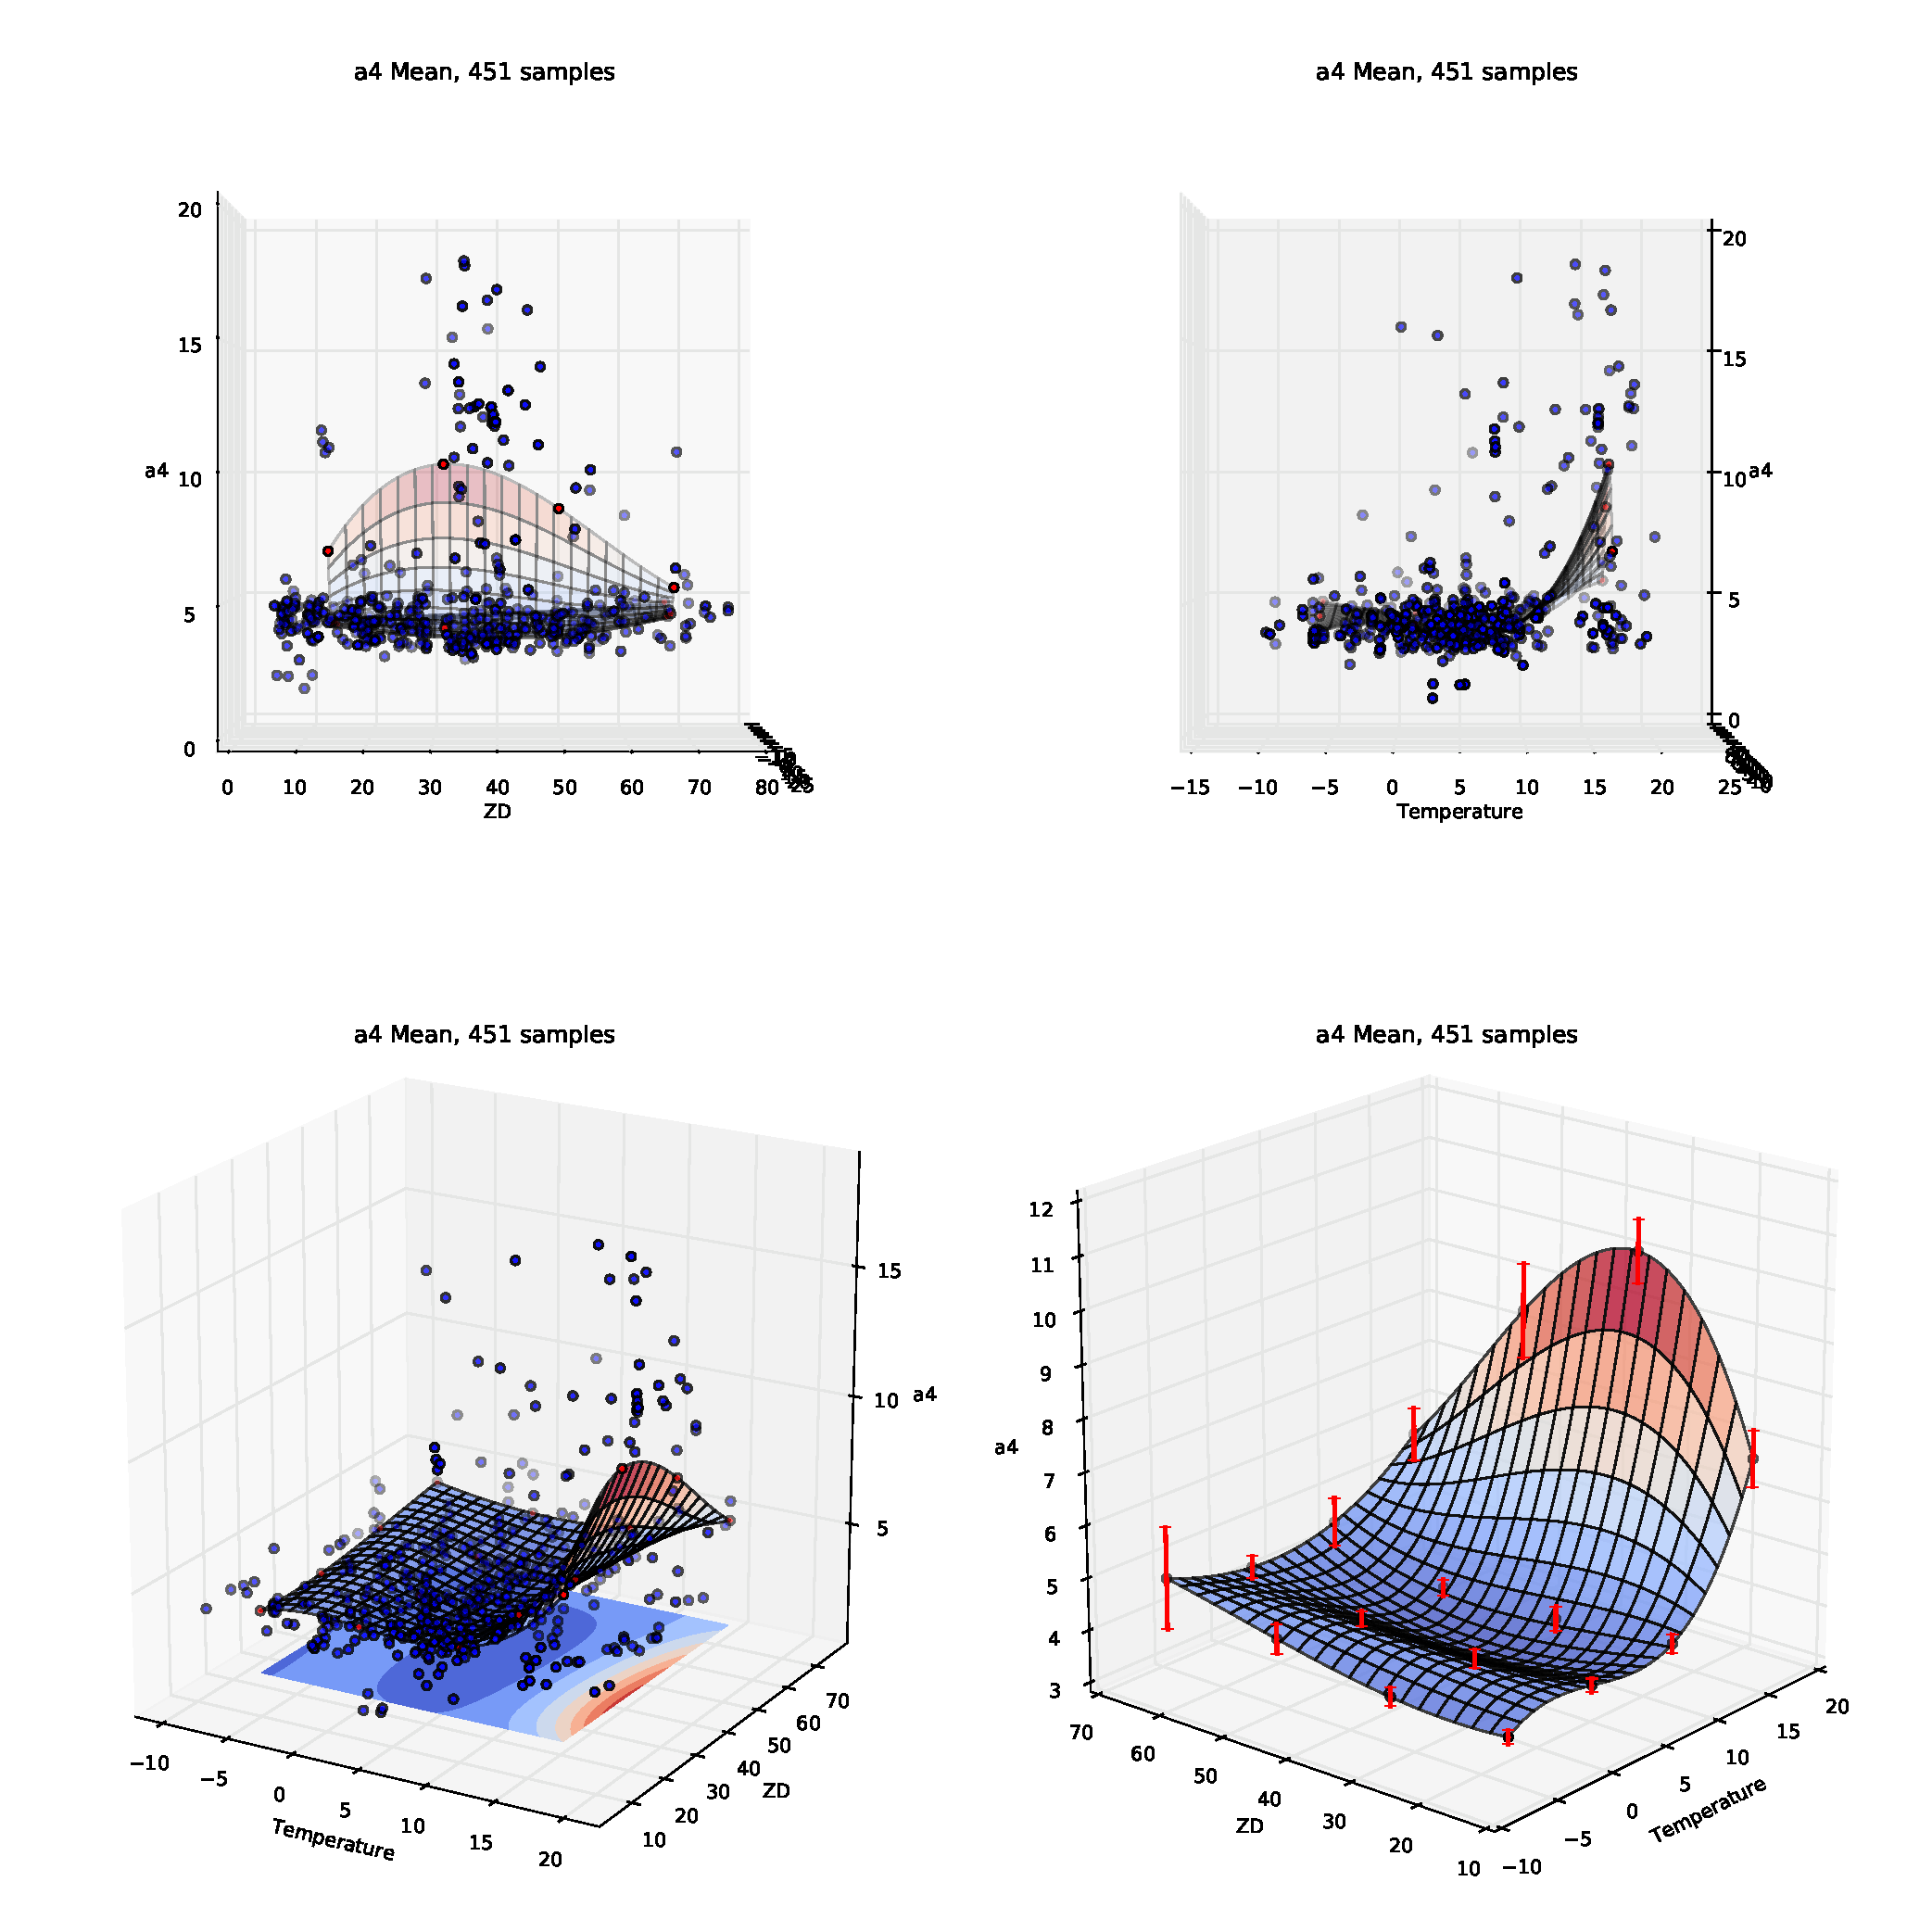
\includegraphics[scale=.48]{psf_surf/a4_mean.pdf}
	\caption[Temperatur- und Elevationsabhängigkeit von $A_4$]{Temperatur- und Elevationsabhängigkeit von $A_4$. Es liegen 451 Fokusaufnahmen zugrunde, die jeweils einem blauen Punkt entsprechen. Die Plots oben links und rechts entsprechen der Projektion auf die Temperatur- und Elevations-Achse respektive. Die roten Kontrollpunkt wurden als Durchschnittswerte berechnet (mean). Die roten Balken an den Kontrollpunkten im Plot unten rechts sind ein Maß für die Streuung des Kontrollpunktes. }
    \label{a4_surf}
\end{figure}

\begin{figure}[h]
	\centering
	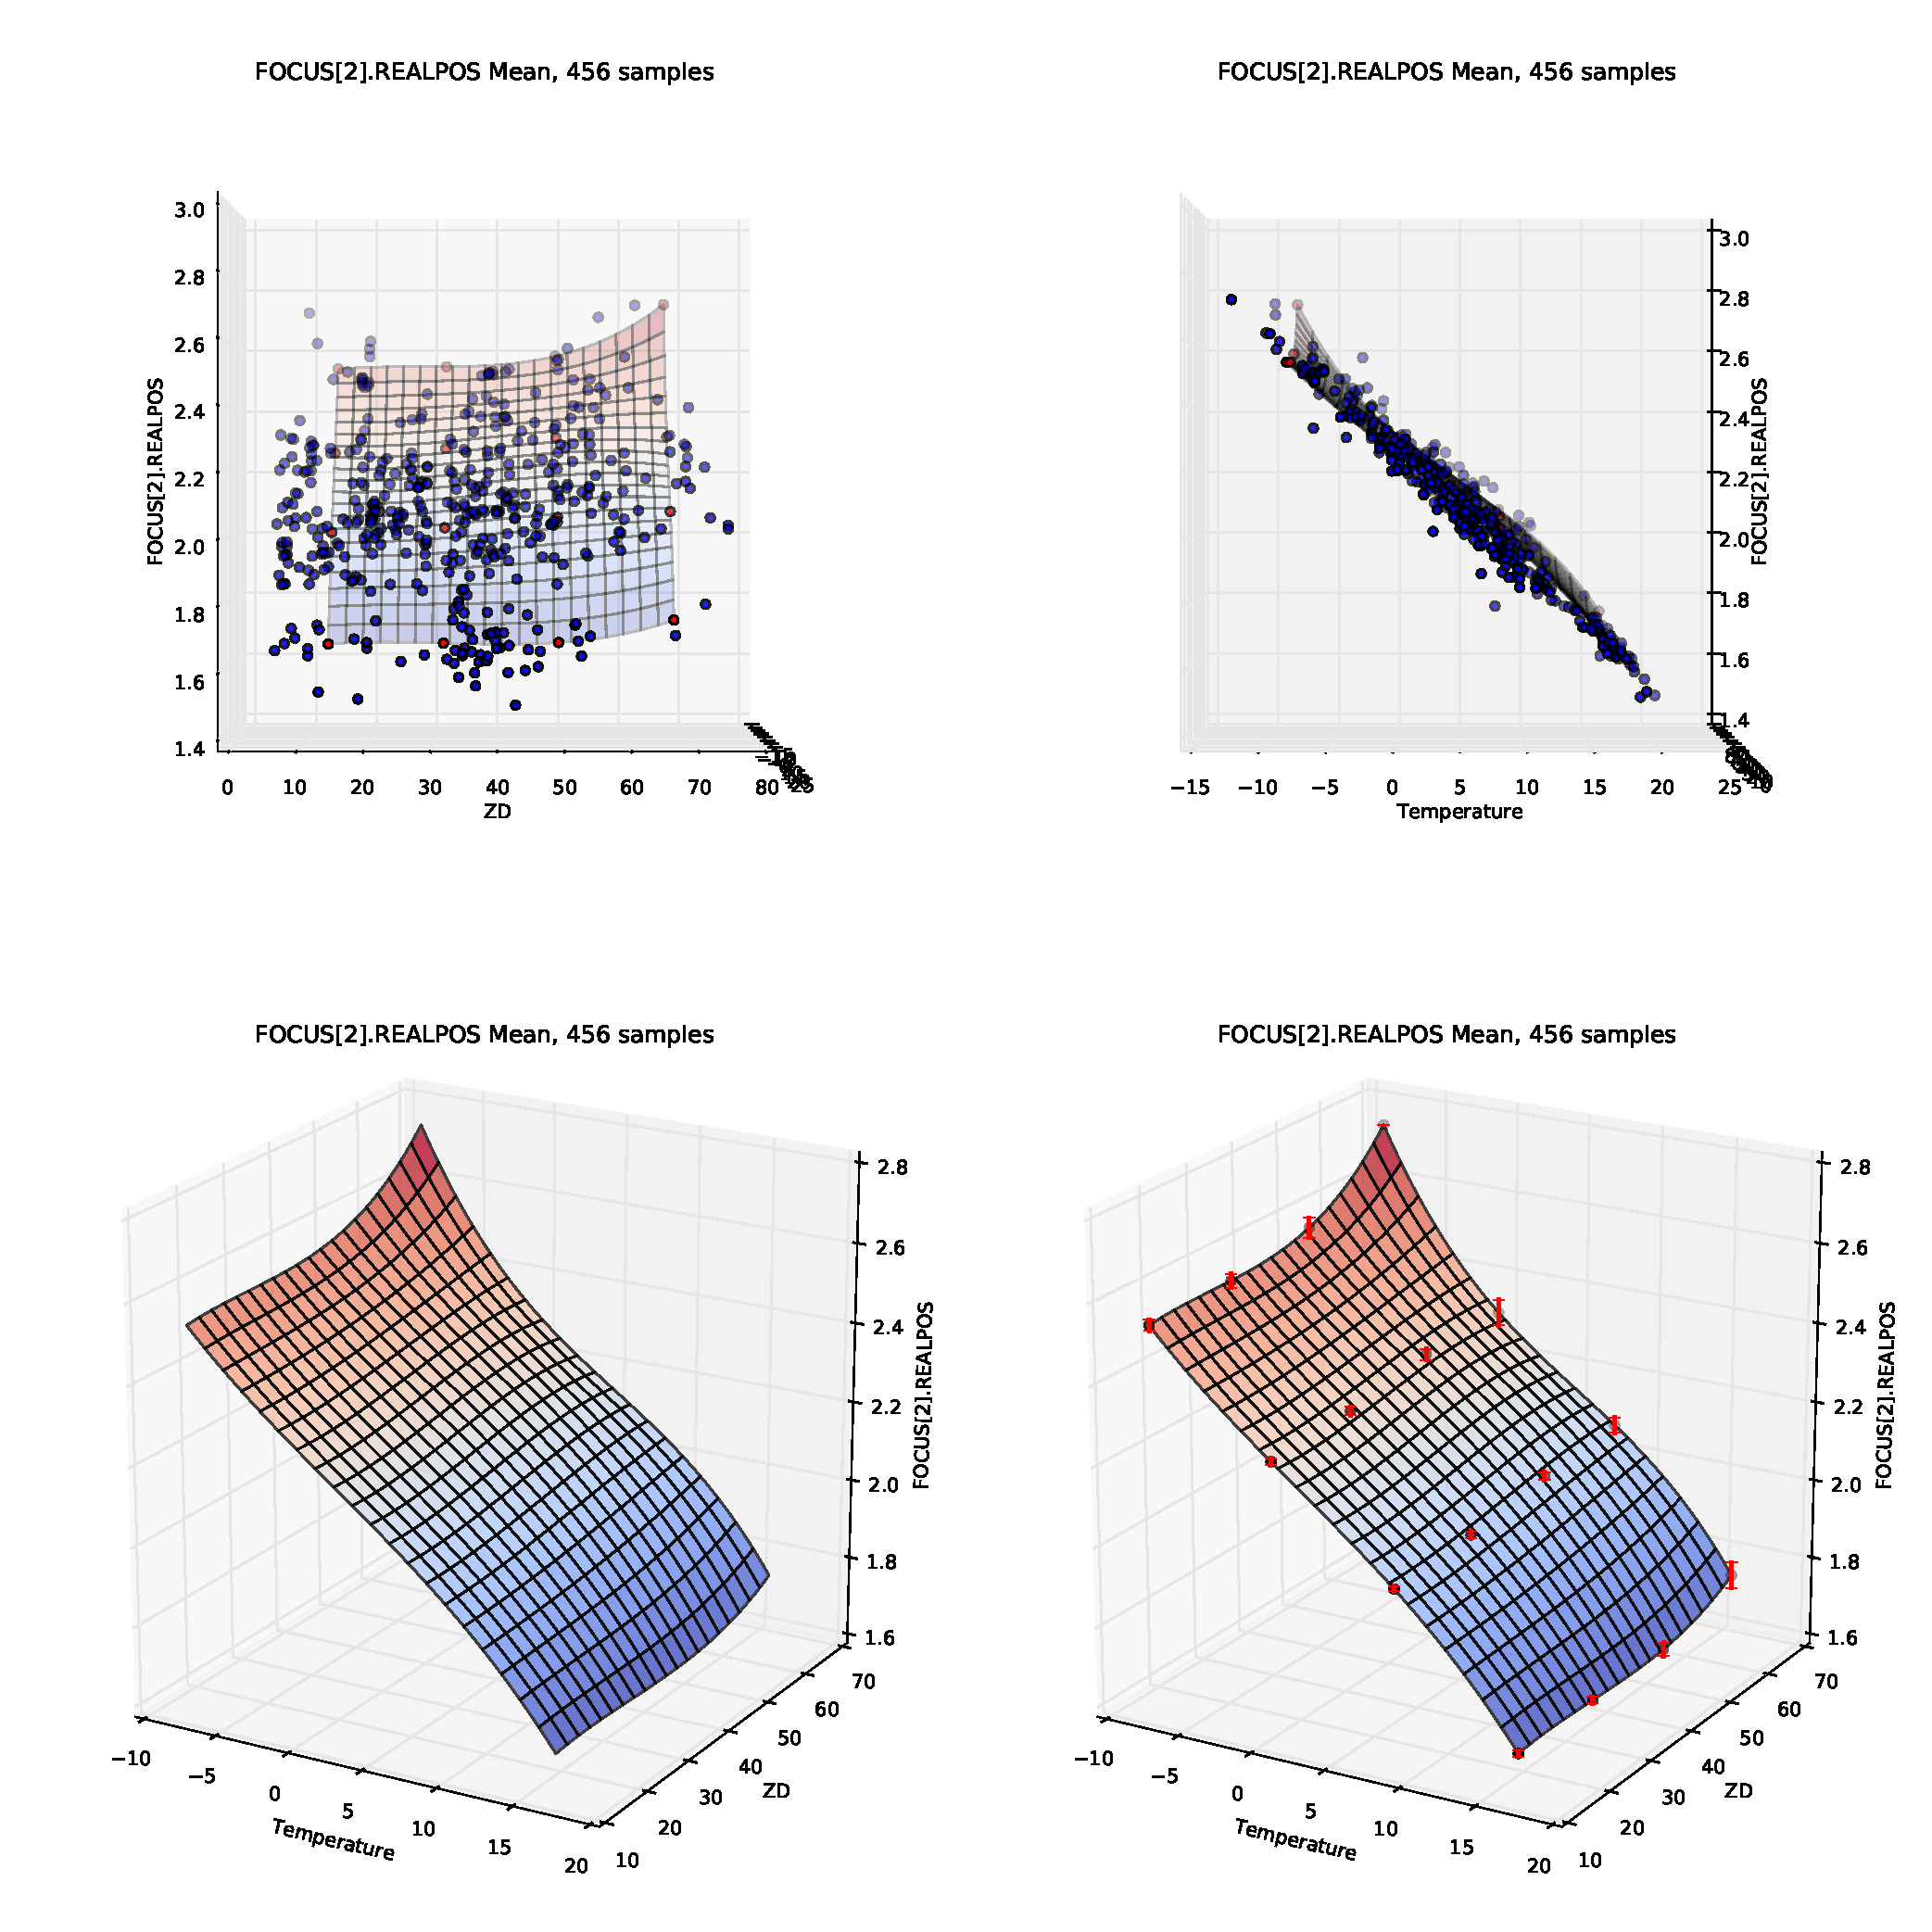
\includegraphics[scale=.45]{tsi_surf/POSITION_INSTRUMENTAL_FOCUS_2__REALPOS_mean.pdf}
	\caption[Temperatur- und Elevationsabhängigkeit der Sekundärspiegelposition]{Temperatur- und Elevationsabhängigkeit der Sekundärspiegelposition entlang der optischen Achse. Die Sekundärspiegelposition von 456 Fokusaufnahmen entsprechen den blauen Punkten. Die roten Kontrollpunkte im Plot unten rechts wurden über den Median aller Punkte in ihrer Umgebung gebildet und enthalten einen roten Fehlerbalken.}

    \label{focus_surf}
\end{figure}
